%========================================================================================
%   Clase 10: Reduccion de dimensionalidad (PCA)
%   Analitica de Datos - Maestria en Ciencias del Comportamiento (UdeSA)
%   Plantilla: SimpleDarkBlue con primario UdeSA + logo institucional
%========================================================================================
\documentclass[aspectratio=169,xcolor=dvipsnames]{beamer}
\usetheme{SimpleDarkBlue}
\useoutertheme[subsection=false]{miniframes}  % navegacion de circulos (uno por slide, por seccion)

\usepackage[utf8]{inputenc}
\usepackage[T1]{fontenc}
\usepackage[spanish,es-noshorthands]{babel}
\usepackage{graphicx}
\usepackage{booktabs}
\usepackage{listings}
\usepackage{tikz}

\usepackage[scaled]{helvet}
\renewcommand{\familydefault}{\sfdefault}

\graphicspath{{./}}

% --- Estilo de codigo Python (listings) ---
\lstdefinestyle{py}{%
    language=Python,
    basicstyle=\ttfamily\footnotesize,
    keywordstyle=\color{udesaNavy}\bfseries,
    commentstyle=\color{tabGray}\itshape,
    stringstyle=\color{tabGreen},
    showstringspaces=false,
    backgroundcolor=\color{blockBodyBg},
    frame=none,
    xleftmargin=0.6em, framexleftmargin=0.6em,
    breaklines=true, columns=fullflexible, keepspaces=true,
    aboveskip=0.5em, belowskip=0.3em,
}
\lstset{style=py}

% --- Primario UdeSA; secundarios = paleta del skill (tab20c) ---
\definecolor{udesaNavy}{HTML}{00529B}
\definecolor{tabBlue}{HTML}{3182BD}
\definecolor{tabOrange}{HTML}{E6550D}
\definecolor{tabOrangeLL}{HTML}{FDD0A2}
\definecolor{tabGreen}{HTML}{31A354}
\definecolor{tabGreenLL}{HTML}{C7E9C0}
\definecolor{tabPurple}{HTML}{756BB1}
\definecolor{tabRed}{HTML}{CB181D}
\definecolor{tabBrown}{HTML}{8C6D31}
\definecolor{tabGray}{HTML}{636363}
\definecolor{tabGrayL}{HTML}{969696}
\definecolor{blockBodyBg}{HTML}{ECECEC}

\setbeamercolor{structure}{fg=udesaNavy}
\setbeamercolor{title}{bg=udesaNavy,fg=white}
\setbeamercolor{frametitle}{bg=udesaNavy,fg=white}
\setbeamercolor{block title}{fg=white,bg=udesaNavy}
\setbeamercolor{block body}{fg=black,bg=blockBodyBg}
\setbeamercolor{block title example}{fg=white,bg=tabGreen}
\setbeamercolor{block body example}{fg=black,bg=tabGreenLL}
\setbeamercolor{block title alerted}{fg=white,bg=tabOrange}
\setbeamercolor{block body alerted}{fg=black,bg=tabOrangeLL}
\setbeamercolor{alerted text}{fg=tabOrange}
\setbeamercolor{itemize item}{fg=udesaNavy}
\setbeamercolor{itemize subitem}{fg=udesaNavy}
\setbeamercolor{enumerate item}{fg=udesaNavy}

% --- Tematizacion por bloque: la BARRA de titulo toma el color del bloque ---
\newcommand{\bloque}[1]{%
    \setbeamercolor{frametitle}{bg=#1,fg=white}%
    \setbeamercolor{structure}{fg=#1}%
    \setbeamercolor{alerted text}{fg=#1}%
    \setbeamercolor{itemize item}{fg=#1}%
    \setbeamercolor{itemize subitem}{fg=#1}%
    \setbeamercolor{enumerate item}{fg=#1}%
}
\newcommand{\navytheme}{\bloque{udesaNavy}}

% --- Logo UdeSA (blanco) arriba a la derecha en las slides de contenido ---
\setbeamertemplate{frametitle}{%
    \nointerlineskip
    \begin{beamercolorbox}[wd=\paperwidth,ht=2.7ex,dp=1.3ex,leftskip=0.4cm,rightskip=0.4cm]{frametitle}%
        \usebeamerfont{frametitle}\insertframetitle%
        \hfill\raisebox{-0.2ex}{
\includegraphics[height=2.1ex]{udesa-logo-color-white.png}}%
    \end{beamercolorbox}%
}

% --- Portada ---
\titlegraphic{
\includegraphics[width=0.27\textwidth]{udesa-logo-color.png}}
\makeatletter
\setbeamertemplate{title page}{%
    \vspace{2.0em}
    \begingroup
    \centering
    {\inserttitlegraphic\par}
    \vskip2.0em
    \begin{beamercolorbox}[sep=10pt,center,shadow=true,rounded=true]{title}
        \usebeamerfont{title}\inserttitle\par%
        \ifx\insertsubtitle\@empty\else%
        \vskip0.4em{\large\usebeamercolor[fg]{subtitle}\insertsubtitle\par}%
        \fi%
    \end{beamercolorbox}%
    \vskip1.2em\par
    {\large\textbf{\insertauthor}\par}%
    \vskip0.25em
    {\small\insertdate\par}%
    \endgroup
    \vfill
}
\makeatother

% --- Navegacion: un circulo por slide, agrupados por bloque ---
\AtBeginSection{}
\setbeamertemplate{headline}{}
\setbeamercolor{mini frame}{fg=gray!55, bg=white}
\setbeamercolor{mini frame in current subsection}{use=structure, fg=structure.fg, bg=structure.fg!30}
\setbeamercolor{mini frame in other subsection}{fg=gray!55, bg=white}
\setbeamercolor{section in head/foot}{fg=gray!60}
\setbeamercolor{subsection in head/foot}{fg=gray!60}
\setbeamertemplate{footline}{%
    \ifnum\insertsectionnumber>0%
        \vskip2pt%
        \hbox to\paperwidth{%
            \hskip0.5cm%
            \raisebox{0.2ex}{\insertnavigation{\dimexpr\paperwidth-1cm\relax}}%
            \hss%
        }%
        \vskip3pt%
    \fi%
}

\title{Clase 10:\\ \textbf{Reducci\'on de dimensionalidad (PCA)}}
\subtitle{Anal\'itica de Datos}
\author{Maestr\'ia en Ciencias del Comportamiento}
\date{Primavera 2026}

\begin{document}

%======================= APERTURA =======================
\navytheme

% -- 1. Portada --
\begin{frame}[plain]\titlepage\end{frame}

% -- 2. Pregunta guia --
\begin{frame}{}
    \vfill
    \begin{center}
        {\Large Medimos \textbf{ocho cosas} de cada estudiante.}\\[0.7em]
        {\Large ?`Se pueden resumir en \alert{una sola}?}\\[1.0em]
        {\footnotesize Datos reales de \textbf{4.424 estudiantes} de educaci\'on superior: notas, materias inscriptas y aprobadas en dos semestres, nota de admisi\'on y edad de ingreso.}\\[0.5em]
        {\footnotesize Vamos a ver que la respuesta es \textbf{s\'i}, y que ese \'unico n\'umero termina diciendo qui\'en abandona.}
    \end{center}
    \vfill
\end{frame}

% -- 3. Roadmap --
\begin{frame}{De qu\'e vamos a hablar hoy}
    \begin{block}{Objetivo}
        Entender el \textbf{an\'alisis de componentes principales (PCA)}: qu\'e hace, c\'omo se lee, cu\'anta informaci\'on conserva y d\'onde conviene usarlo en Ciencias del Comportamiento.
    \end{block}
    \begin{enumerate}\footnotesize
        \item \textbf{Por qu\'e reducir.} Muchas variables correlacionadas esconden pocas dimensiones.
        \item \textbf{Qu\'e es una componente.} De la intuici\'on en 2D al caso de $p$ variables.
        \item \textbf{Leer el resultado.} El biplot y c\'omo se interpretan sus flechas.
        \item \textbf{Cu\'anta informaci\'on conservamos.} Reconstrucci\'on, varianza explicada y scree plot.
        \item \textbf{Decisiones y alcance.} Estandarizar, m\'etodos no lineales y casos aplicados.
        \item \textbf{Supuestos y l\'imites.} Qu\'e asume PCA y cu\'ando no corresponde.
    \end{enumerate}
    \vfill
    \begin{center}
        {\footnotesize Para la pr\'actica vamos a~\href{https://colab.research.google.com/github/tomdamelio/analitica_de_datos/blob/main/clases/clase-10/notebooks/clase10_python.ipynb}{\raisebox{-0.32\height}{
\includegraphics[height=3.4ex]{colab_logo.png}}~\textbf{Colab}}.}
    \end{center}
\end{frame}

%======================= BLOQUE 1 =======================
\section{Por qu\'e reducir}
\bloque{tabBlue}

\begin{frame}{}
    \vfill
    \begin{center}
        {\small\textbf{\color{tabBlue}BLOQUE 1 DE 6}}\\[0.5em]
        {\Large\textbf{Por qu\'e reducir}}\\[0.8em]
        {\normalsize Cuando hay demasiadas variables para mirarlas.}
    \end{center}
    \vfill
\end{frame}

\begin{frame}{Aprendizaje no supervisado: no hay qu\'e predecir}
    \begin{itemize}
        \item Hasta ahora tuvimos siempre una variable respuesta $Y$. Ac\'a \textbf{no la hay}: solo un conjunto de features $X_1,\dots,X_p$.
        \item El objetivo cambia: ya no es predecir, es \alert{descubrir estructura} en los datos.
        \item Por eso el an\'alisis no supervisado casi siempre es parte de un \textbf{an\'alisis exploratorio}.
        \item Y por eso mismo es m\'as \textbf{subjetivo}: no hay una respuesta correcta contra la cual validar, ni test set que nos diga si acertamos.
    \end{itemize}
    \vfill
    {\footnotesize ISLP, Secci\'on 12.1.}
\end{frame}

\begin{frame}{Agrupar clientes que nadie etiquet\'o}
    \begin{exampleblock}{Un caso cotidiano}
        Un sitio de compras online quiere recomendarle a cada persona lo que le interesa. Agrupa a sus clientes seg\'un su \textbf{historial de navegaci\'on y compra}, sin que nadie haya dicho de antemano a qu\'e grupo pertenece cada uno.
    \end{exampleblock}
    \begin{itemize}
        \item Nadie defini\'o los grupos: \textbf{emergen de los datos}.
        \item Un buscador hace lo mismo con historiales de clics para decidir qu\'e resultados mostrar.
        \item PCA ataca una versi\'on de ese problema: cuando hay \textbf{muchas variables correlacionadas}, resumirlas en unas pocas que conserven casi toda la variabilidad.
    \end{itemize}
\end{frame}

\begin{frame}{Varias variables dicen casi lo mismo}
    \centering
    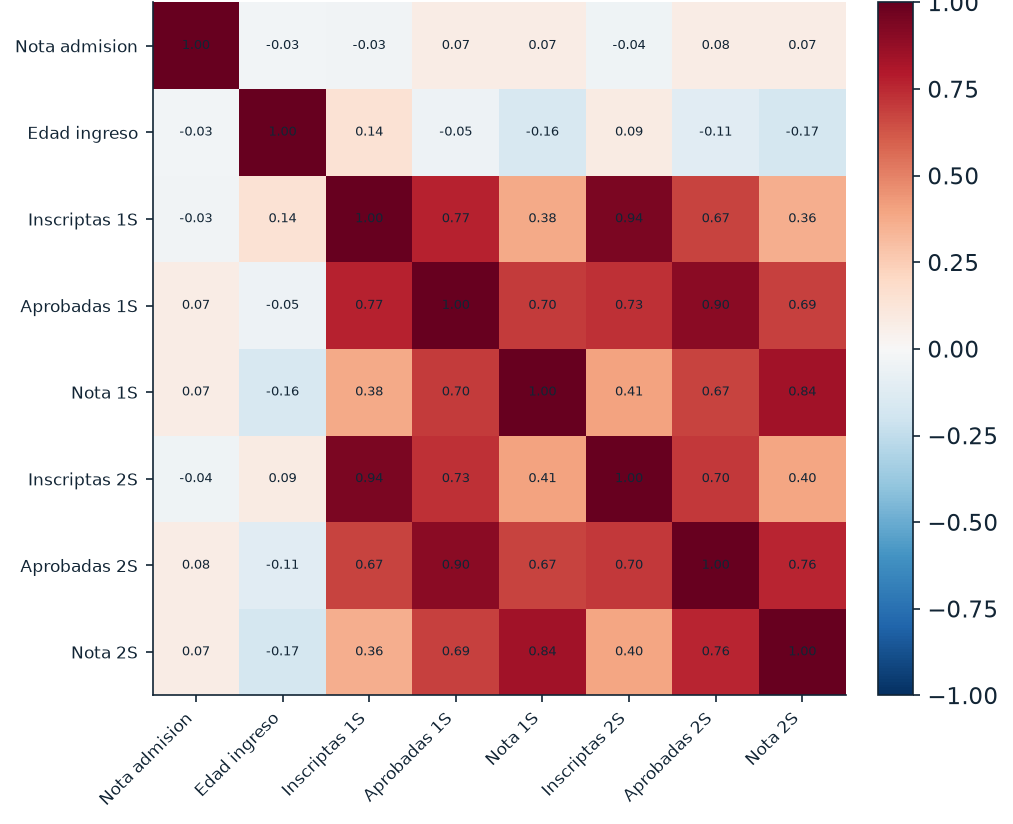
\includegraphics[width=\linewidth,height=0.70\textheight,keepaspectratio]{clase10_correlaciones_notitle.png}\\
    {\footnotesize Correlaciones del bloque acad\'emico. Las materias \textbf{aprobadas en 1er y 2do semestre} correlacionan \textbf{0,90}: quien aprueba mucho en un semestre aprueba mucho en el otro. Hay \alert{redundancia} para explotar.}
\end{frame}

\begin{frame}{Con 8 variables ya hay 28 gr\'aficos posibles}
    \begin{itemize}
        \item Para mirar las relaciones de a pares hacen falta $p(p-1)/2$ diagramas de dispersi\'on.
        \item Con nuestras \textbf{8 variables} son \textbf{28} gr\'aficos. Con las \textbf{24} columnas num\'ericas del dataset, \alert{276}.
        \item Ninguno muestra la foto completa: cada uno contiene solo una fracci\'on de la informaci\'on.
    \end{itemize}
    \vfill
    \begin{alertblock}{La pregunta que abre PCA}
        ?`Existe una representaci\'on de \textbf{pocas dimensiones} que capture la mayor parte posible de la variabilidad de los datos?
    \end{alertblock}
\end{frame}

\begin{frame}{De 4.500 adjetivos a cinco factores}
    \begin{itemize}
        \item En 1936, Allport y Odbert listaron \textbf{4.500 t\'erminos} que describen diferencias de personalidad.
        \item Con an\'alisis factorial (el pariente cercano de PCA), esos t\'erminos se redujeron primero a 16 y finalmente a \alert{cinco}: el modelo \textbf{Big Five} (OCEAN).
        \item De Raad y Barelds (2008) aplicaron PCA a \textbf{2.365 \'items} del l\'exico holand\'es y recuperaron el Big Five m\'as tres factores adicionales.
    \end{itemize}
    \vfill
    \begin{block}{El principio, en una l\'inea}
        Con $p$ enorme, unas pocas \textbf{dimensiones compuestas} pueden resumir una variedad inmensa. Es exactamente lo que vamos a hacer hoy, en menor escala.
    \end{block}
\end{frame}

%======================= BLOQUE 2 =======================
\section{Qu\'e es una componente}
\bloque{tabOrange}

\begin{frame}{}
    \vfill
    \begin{center}
        {\small\textbf{\color{tabOrange}BLOQUE 2 DE 6}}\\[0.5em]
        {\Large\textbf{Qu\'e es una componente principal}}\\[0.8em]
        {\normalsize De la intuici\'on en dos dimensiones al caso general.}
    \end{center}
    \vfill
\end{frame}

\begin{frame}{En 2D: la direcci\'on de m\'axima varianza}
    \centering
    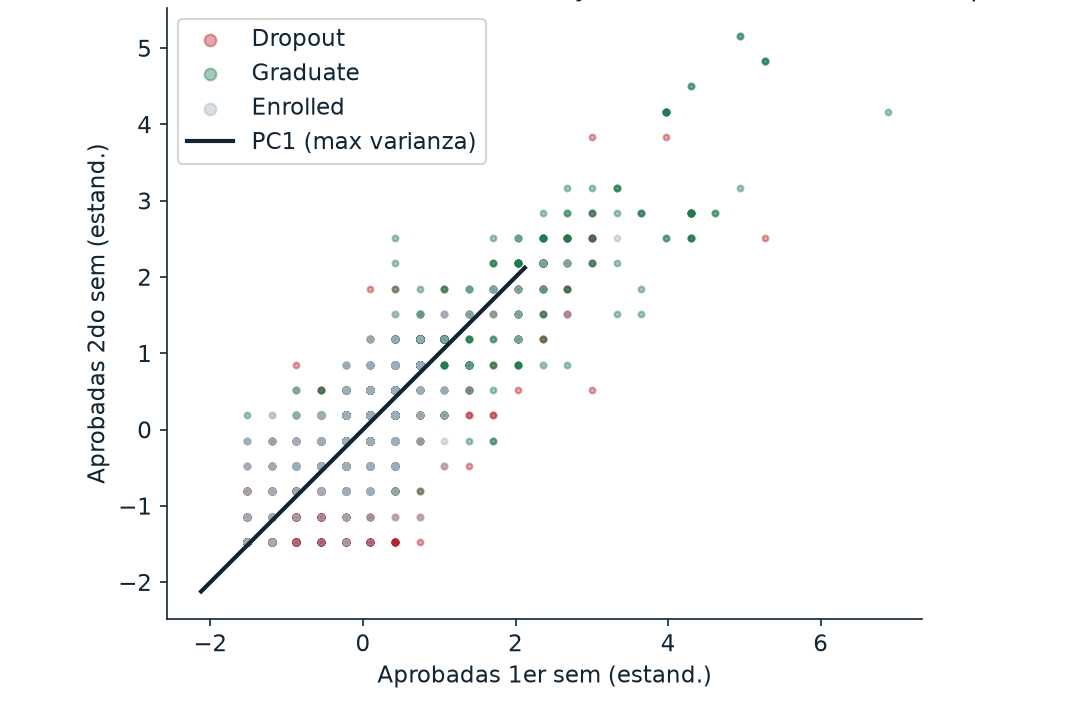
\includegraphics[width=\linewidth,height=0.70\textheight,keepaspectratio]{clase10_pca2d_notitle.png}\\
    {\footnotesize Materias aprobadas en 1er y 2do semestre (estandarizadas). La recta negra es la \textbf{primera componente}: la direcci\'on a lo largo de la cual los puntos var\'ian m\'as. Ella sola concentra el \alert{95,2\%} de la variabilidad de las dos variables.}
\end{frame}

\begin{frame}{...y a la vez la recta m\'as cercana a los puntos}
    \centering
    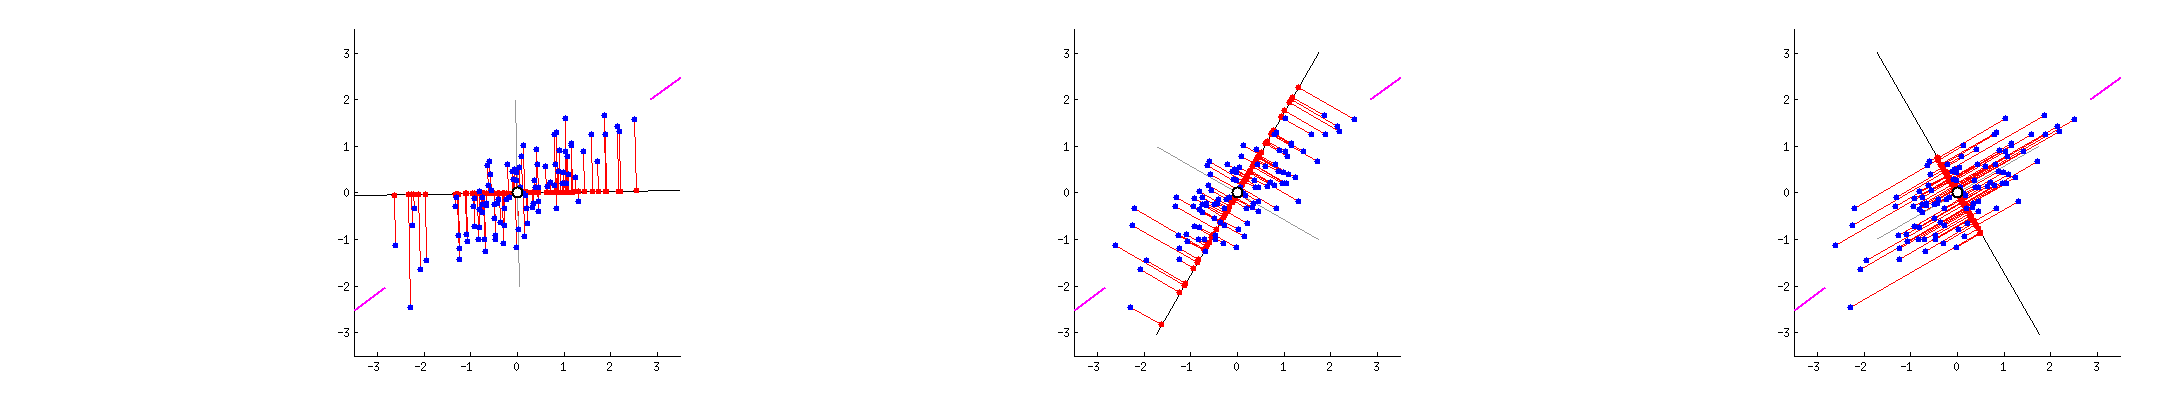
\includegraphics[width=\linewidth,height=0.66\textheight,keepaspectratio]{gif_errores_tira.png}\\
    {\footnotesize La misma recta girando. Los \textbf{segmentos rojos} son los errores de proyecci\'on. Cuando la recta llega a la primera componente, esos errores alcanzan su \textbf{m\'inimo} y, en ese mismo instante, las proyecciones quedan \alert{lo m\'as dispersas posible}.}
\end{frame}

\begin{frame}{Dos lecturas del mismo problema}
    \begin{columns}[t]
        \begin{column}{0.48\textwidth}
            \begin{block}{M\'axima varianza}
                La direcci\'on a lo largo de la cual los datos proyectados tienen la \textbf{mayor dispersi\'on} posible.
            \end{block}
        \end{column}
        \begin{column}{0.48\textwidth}
            \begin{exampleblock}{M\'inima distancia}
                La recta que \textbf{minimiza} la suma de distancias al cuadrado entre cada punto y su proyecci\'on.
            \end{exampleblock}
        \end{column}
    \end{columns}
    \vskip1.0em
    \begin{itemize}
        \item Las dos definiciones llevan a la \alert{misma soluci\'on matem\'atica}.
        \item No es casualidad: la varianza total es fija, as\'i que todo lo que la proyecci\'on captura es exactamente lo que el error deja de perder.
        \item Volvemos sobre esto en el Bloque 4, ya con n\'umeros.
    \end{itemize}
\end{frame}

\begin{frame}{En 3D: dos componentes definen un plano}
    \centering
    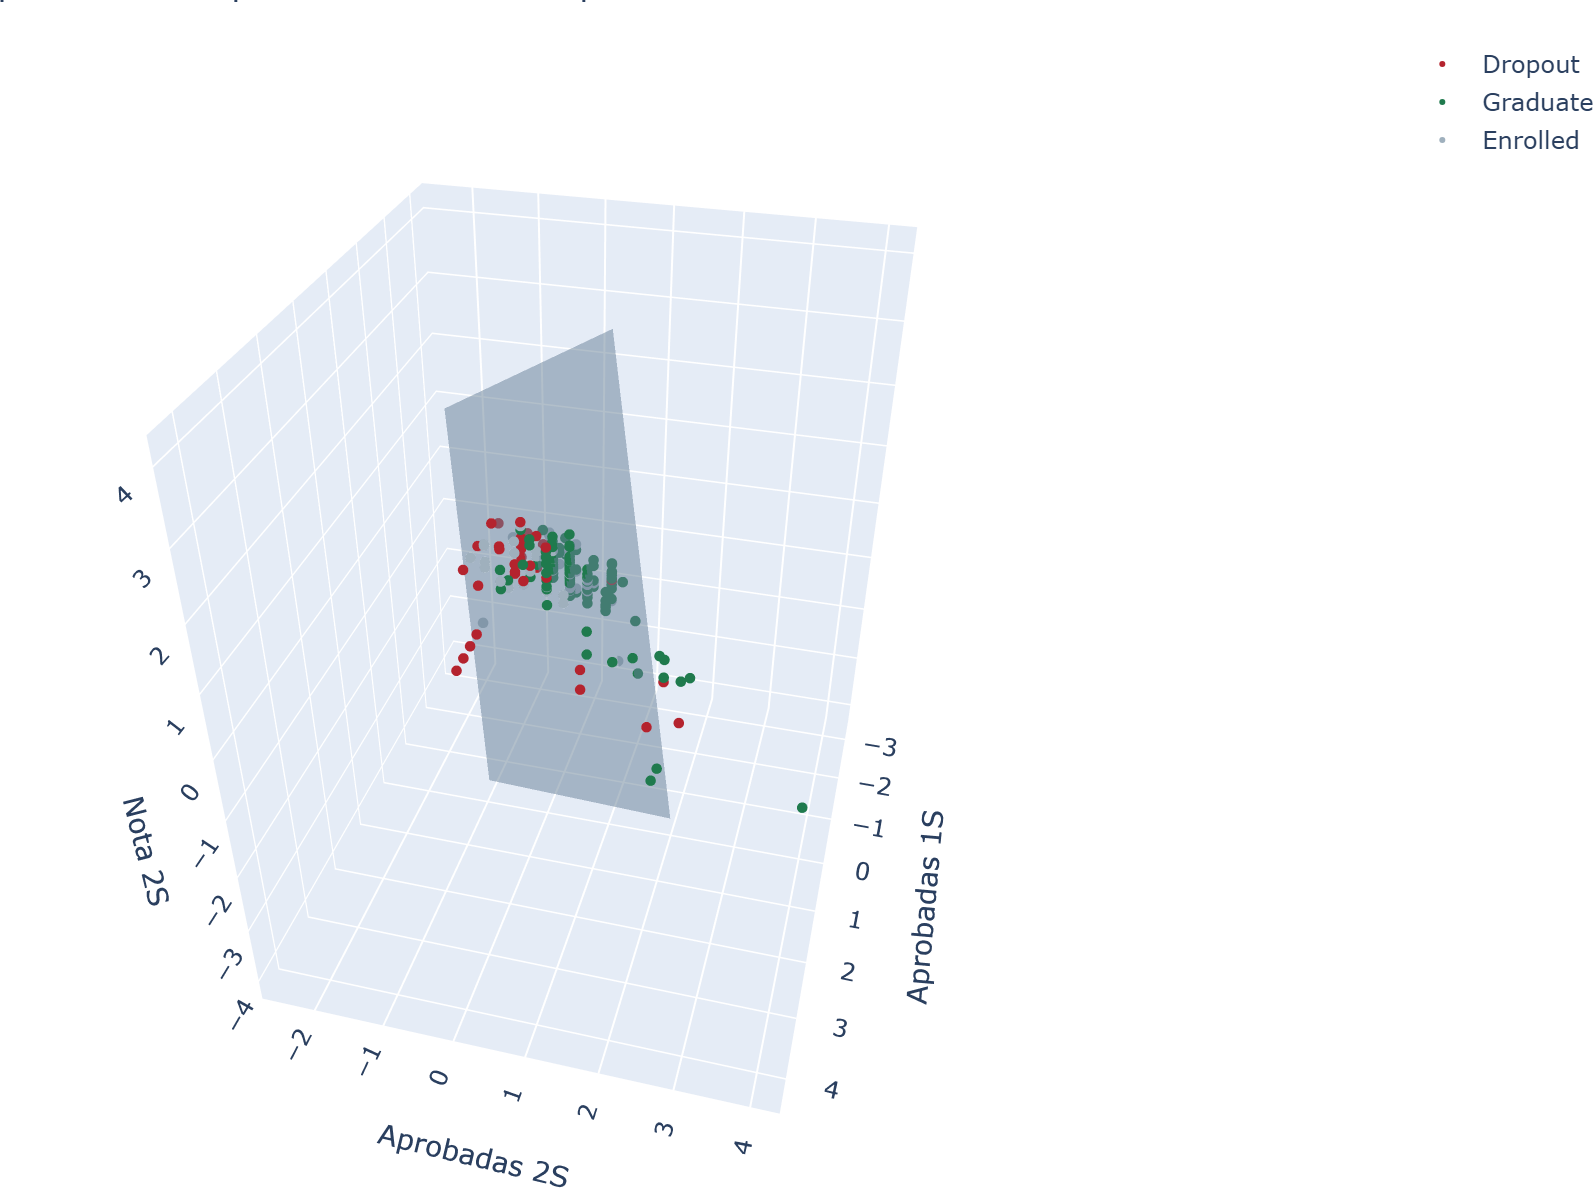
\includegraphics[width=\linewidth,height=0.70\textheight,keepaspectratio]{clase10_3d_notitle.png}\\
    {\footnotesize Tres variables acad\'emicas. Las \textbf{dos primeras componentes} generan el plano que mejor se apoya sobre la nube. Con $p$ variables la idea es la misma: un subespacio de pocas dimensiones, lo m\'as cerca posible de los datos.}
\end{frame}

\begin{frame}{Una componente es una combinaci\'on lineal}
    Cada componente es una \textbf{variable nueva}, construida ponderando las originales:
    \vskip0.4em
    \begin{center}
        $Z_m = \phi_{1m} X_1 + \phi_{2m} X_2 + \cdots + \phi_{pm} X_p$
    \end{center}
    \vskip0.4em
    donde:
    \begin{itemize}\footnotesize
        \item $X_1,\dots,X_p$ son las variables originales, ya centradas en media cero;
        \item los \textbf{\emph{loadings}} $\phi_{jm}$ son los \alert{pesos}: cu\'anto aporta cada variable a la componente $m$;
        \item los \textbf{\emph{scores}} $Z_m$ son los \alert{valores} resultantes: la posici\'on de cada estudiante en esa nueva variable.
    \end{itemize}
    \vskip0.5em
    {\footnotesize Los loadings describen \textbf{variables}; los scores describen \textbf{observaciones}. Es la distinci\'on que hace legible un biplot.}
\end{frame}

\begin{frame}{Por qu\'e los pesos se normalizan}
    \begin{itemize}
        \item Se exige que la suma de los cuadrados de los pesos sea \textbf{igual a 1}.
        \item Sin esa restricci\'on el problema \alert{no tendr\'ia soluci\'on}: agrandando los pesos, la varianza crecer\'ia sin l\'imite.
        \item Normalizar obliga a buscar una \textbf{direcci\'on} en el espacio de las variables, no una magnitud arbitraria.
    \end{itemize}
    \vfill
    \begin{block}{C\'omo se calcula en la pr\'actica}
        Los pesos salen de la \textbf{descomposici\'on en autovectores y autovalores} de la matriz de covarianzas (o de correlaciones, si estandarizamos). Cada componente es un \textbf{autovector}; la varianza que explica es su \textbf{autovalor}. No hace falta resolverlo a mano: lo hace la funci\'on de PCA.
    \end{block}
\end{frame}

\begin{frame}{Cada componente es ortogonal a las anteriores}
    \begin{itemize}
        \item La segunda componente se busca igual que la primera, maximizando varianza, pero con una condici\'on extra: ser \alert{ortogonal} (no correlacionada) con la primera.
        \item Lo mismo para la tercera respecto de las dos anteriores, y as\'i sucesivamente.
        \item Cada una captura \textbf{informaci\'on nueva}, no una repetici\'on de la anterior.
        \item En total hay como m\'aximo $\min(n-1,\; p)$ componentes. Con nuestras 8 variables, \textbf{8 componentes}.
    \end{itemize}
    \vfill
    {\footnotesize Usar \emph{todas} las componentes no pierde nada: es solo \textbf{rotar} el sistema de coordenadas. La compresi\'on aparece cuando nos quedamos con algunas.}
\end{frame}

\begin{frame}{El score de un estudiante, t\'ermino a t\'ermino}
    \centering
    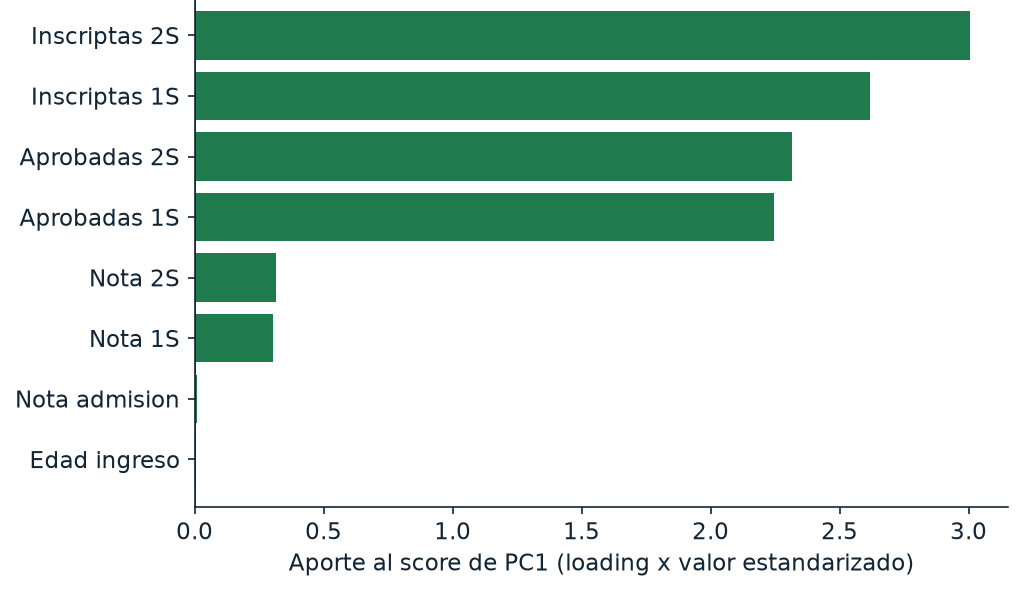
\includegraphics[width=\linewidth,height=0.66\textheight,keepaspectratio]{clase10_score_termino_notitle.png}\\
    {\footnotesize Aporte de cada variable al score en PC1 de un estudiante concreto: su \textbf{valor estandarizado por el loading} de esa variable. Las cuatro variables de \alert{materias} explican casi todo el score; la nota de admisi\'on y la edad, pr\'acticamente nada.}
\end{frame}

\begin{frame}{Las componentes est\'an definidas salvo el signo}
    \begin{alertblock}{Un detalle que confunde}
        Dos programas pueden devolver la \textbf{misma componente con el signo invertido}, y ambos son correctos.
    \end{alertblock}
    \begin{itemize}
        \item Un vector de pesos define una \textbf{direcci\'on}, y una direcci\'on se extiende hacia los dos lados.
        \item Dar vuelta el signo de los loadings y el de los scores a la vez deja \textbf{todo igual}.
        \item Lo que importa es la \textbf{geometr\'ia relativa}: qu\'e variables van juntas y cu\'ales se oponen.
        \item En la pr\'actica conviene \textbf{orientar} cada componente para que se lea bien, como hicimos al poner el \'exito acad\'emico hacia la derecha.
    \end{itemize}
\end{frame}

\begin{frame}{}
    \vfill
    \begin{center}
        \href{https://colab.research.google.com/github/tomdamelio/analitica_de_datos/blob/main/clases/clase-10/notebooks/clase10_python.ipynb}{
\includegraphics[height=7ex]{colab_logo.png}}\\[0.6em]
        {\Large\textbf{A la notebook}}\\[0.6em]
        {\normalsize Calcular un score \textbf{a mano} y comprobar que coincide con el del algoritmo.}\\[0.4em]
        {\footnotesize Tambi\'en: rotar la recta y ver c\'omo cambia la varianza proyectada.}
    \end{center}
    \vfill
\end{frame}

%======================= BLOQUE 3 =======================
\section{Leer el biplot}
\bloque{tabGreen}

\begin{frame}{}
    \vfill
    \begin{center}
        {\small\textbf{\color{tabGreen}BLOQUE 3 DE 6}}\\[0.5em]
        {\Large\textbf{Leer el resultado: el biplot}}\\[0.8em]
        {\normalsize Observaciones y variables, en un mismo gr\'afico.}
    \end{center}
    \vfill
\end{frame}

\begin{frame}{El biplot: scores y loadings a la vez}
    \centering
    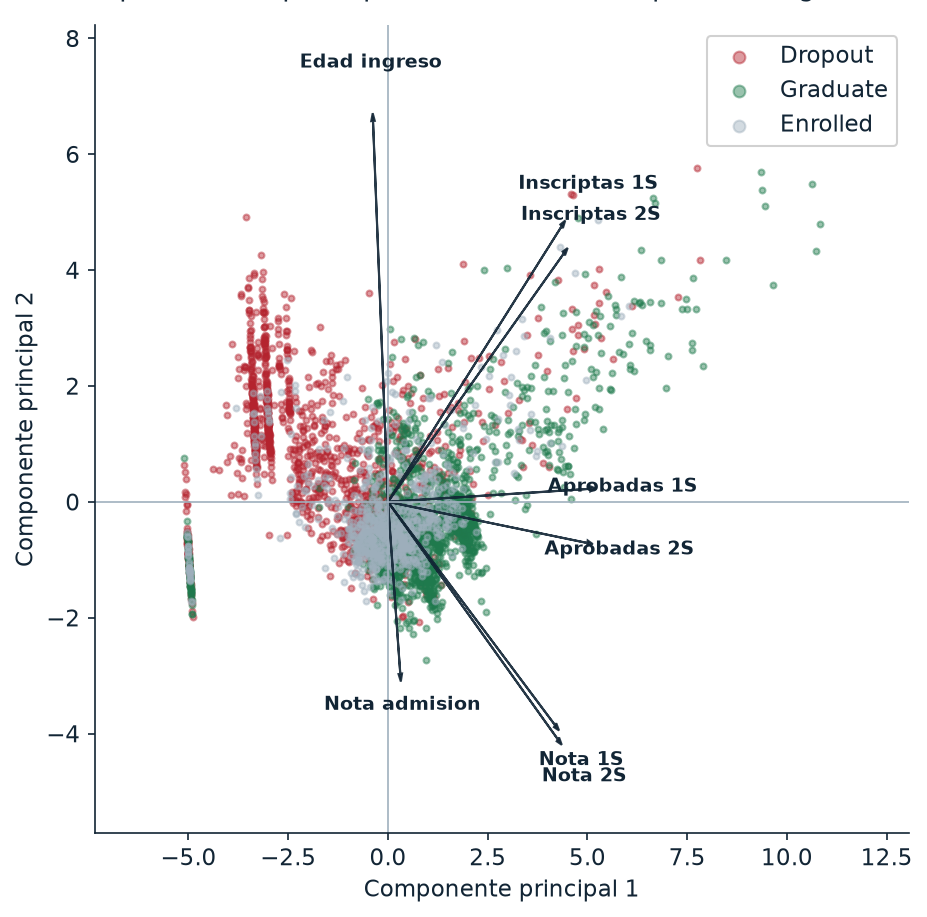
\includegraphics[width=\linewidth,height=0.70\textheight,keepaspectratio]{clase10_biplot_notitle.png}\\
    {\footnotesize Dos gr\'aficos superpuestos: los \textbf{puntos} son estudiantes (scores) y las \textbf{flechas} son variables (loadings), cada uno con su escala. Las dos primeras componentes resumen el \alert{71,5\%} de la variabilidad de las ocho variables.}
\end{frame}

\begin{frame}{PC1 result\'o un eje de riesgo acad\'emico}
    \begin{block}{El hallazgo}
        PCA \textbf{nunca vio} la etiqueta de deserci\'on. Aun as\'i, la primera componente separa a quienes abandonan de quienes se grad\'uan.
    \end{block}
    \begin{itemize}
        \item Score medio en PC1: \textbf{+0,96} entre quienes se grad\'uan, \textbf{--1,43} entre quienes desertan.
        \item PC1 sola explica el \alert{54,2\%} de la variabilidad de las ocho variables.
        \item Las variables de \textbf{materias} son las que definen ese eje; la nota de admisi\'on casi no participa.
    \end{itemize}
    \vskip0.4em
    {\footnotesize Es el mismo tipo de lectura con la que el libro interpreta que la PC1 de \texttt{USArrests} mide criminalidad general.}
\end{frame}

\begin{frame}{C\'omo se leen las flechas: direcci\'on}
    \begin{itemize}
        \item La \textbf{direcci\'on} de una flecha dice qu\'e mezcla de PC1 y PC2 representa a esa variable.
        \item Flecha casi \textbf{horizontal}: la variable carga sobre la primera componente. Casi \textbf{vertical}: sobre la segunda.
        \item Es lo que permite ponerle \alert{nombre sustantivo} a cada eje.
    \end{itemize}
    \vfill
    \begin{exampleblock}{En nuestro biplot}
        Las seis variables de cursada apuntan hacia la \textbf{derecha}, con pesos del mismo signo y magnitud parecida: por eso el eje horizontal se lee como \textbf{rendimiento acad\'emico}. La edad de ingreso y la nota de admisi\'on viven sobre el eje vertical.
    \end{exampleblock}
\end{frame}

\begin{frame}{\'Angulo y longitud: lo que agregan las flechas}
    \begin{columns}[t]
        \begin{column}{0.48\textwidth}
            \begin{block}{\'Angulo entre flechas}
                Aproxima la \textbf{correlaci\'on} entre las variables.
                \begin{itemize}\footnotesize
                    \item Misma direcci\'on: muy correlacionadas.
                    \item Perpendiculares: sin correlaci\'on.
                    \item Opuestas: correlaci\'on negativa.
                \end{itemize}
            \end{block}
        \end{column}
        \begin{column}{0.48\textwidth}
            \begin{exampleblock}{Longitud de la flecha}
                Indica qu\'e tan bien \textbf{representada} queda esa variable en el plano.
                \begin{itemize}\footnotesize
                    \item Larga: el plano la captura bien.
                    \item Corta: vive en las componentes que no estamos mirando.
                \end{itemize}
            \end{exampleblock}
        \end{column}
    \end{columns}
    \vskip0.8em
    \begin{itemize}\footnotesize
        \item Las flechas de \textbf{inscriptas 1S y 2S} son casi paralelas, y su correlaci\'on real es alta: el gr\'afico no miente.
        \item La \textbf{nota de admisi\'on} tiene la flecha m\'as corta: sobre ella el biplot \alert{no autoriza ninguna lectura}.
    \end{itemize}
\end{frame}

\begin{frame}{Nombrar las componentes: un caso de consumo}
    \begin{block}{L\'acteos locales (Apulia, Italia, 2022)}
        Un experimento de elecci\'on online con \textbf{543 encuestados} sobre productos l\'acteos locales: calidad, sustentabilidad y disponibilidad.
    \end{block}
    \begin{itemize}
        \item Aplicaron PCA a las respuestas y quedaron \textbf{cuatro componentes}, que nombraron seg\'un qu\'e \'items cargaban fuerte en cada una: sensibilidad a la calidad, ``lo local es mejor'', ``lo local es sustentable'' y demanda de mayor disponibilidad.
        \item Despu\'es relacionaron esas dimensiones con variables \textbf{sociodemogr\'aficas}.
    \end{itemize}
    \vskip0.3em
    {\footnotesize El flujo t\'ipico en Ciencias del Comportamiento: cuestionario con muchos \'items $\rightarrow$ PCA $\rightarrow$ \alert{nombrar} cada componente $\rightarrow$ relacionarla con otras variables.}
\end{frame}

%======================= BLOQUE 4 =======================
\section{Cu\'anta informaci\'on}
\bloque{tabPurple}

\begin{frame}{}
    \vfill
    \begin{center}
        {\small\textbf{\color{tabPurple}BLOQUE 4 DE 6}}\\[0.5em]
        {\Large\textbf{Cu\'anta informaci\'on conservamos}}\\[0.8em]
        {\normalsize Reconstruir, medir el error y decidir cu\'antas componentes.}
    \end{center}
    \vfill
\end{frame}

\begin{frame}{Reconstruir un dato desde sus componentes}
    Si los scores se armaron combinando las variables, se puede hacer el \textbf{camino inverso}:
    \vskip0.4em
    \begin{center}
        $x_{ij} \;\approx\; \sum_{m=1}^{M} z_{im}\,\phi_{jm}$
    \end{center}
    \vskip0.4em
    donde:
    \begin{itemize}\footnotesize
        \item $x_{ij}$ es el dato original: la variable $j$ del estudiante $i$;
        \item $M$ es cu\'antas componentes usamos. Si $M = p$, la reconstrucci\'on es \textbf{exacta};
        \item $z_{im}$ es el \emph{score} del estudiante $i$ en la componente $m$;
        \item $\phi_{jm}$ es el \emph{loading} de la variable $j$ en esa componente.
    \end{itemize}
    \vskip0.5em
    \begin{block}{Por qu\'e importa}
        Con $M$ componentes, esta es \alert{la mejor aproximaci\'on posible} en $M$ dimensiones. Ninguna otra combinaci\'on lineal reconstruye mejor. Eso es lo que hace de PCA una t\'ecnica de \textbf{compresi\'on}, no un resumen m\'as.
    \end{block}
\end{frame}

\begin{frame}{El error cae r\'apido: pocas componentes bastan}
    \centering
    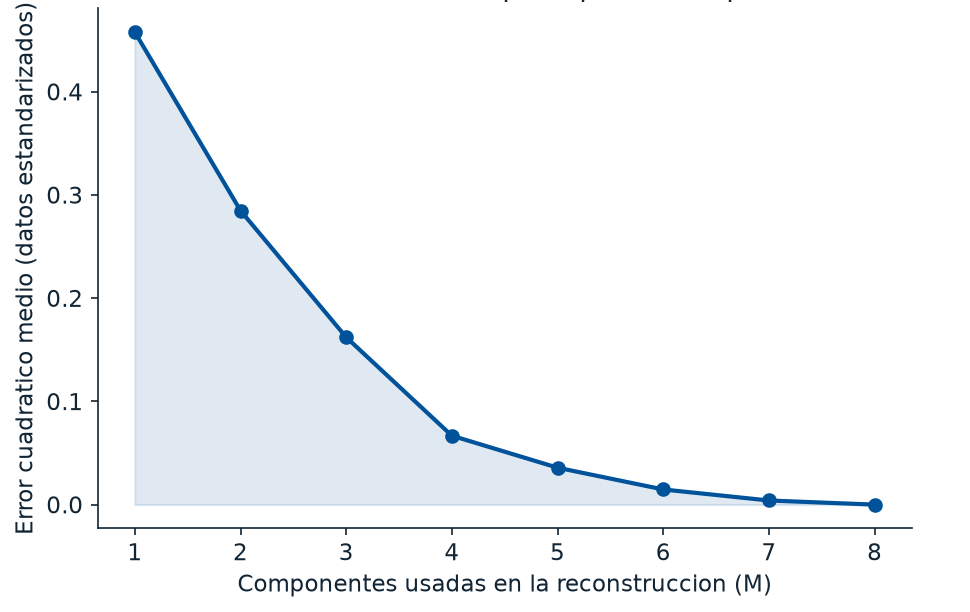
\includegraphics[width=\linewidth,height=0.66\textheight,keepaspectratio]{clase10_reconstruccion_notitle.png}\\
    {\footnotesize Error cuadr\'atico medio al reconstruir las ocho variables de los 4.424 estudiantes. Con \textbf{1} componente es 0,46; con \textbf{4} baja a 0,07; con las \textbf{8} es exactamente \alert{cero}: usar todas es solo rotar los ejes.}
\end{frame}

\begin{frame}{La varianza total se reparte entre las componentes}
    \begin{itemize}
        \item Con variables \textbf{estandarizadas}, cada una aporta 1 unidad de varianza: la varianza total es exactamente $p$ (ac\'a, \textbf{8}).
        \item Cada componente explica una porci\'on de ese total: su \textbf{autovalor}.
        \item La \textbf{PVE} de una componente es esa porci\'on sobre el total. Sumando todas, siempre da 100\%.
    \end{itemize}
    \vskip0.6em
    \begin{center}\footnotesize
    \begin{tabular}{@{}lcccccccc@{}}
        \toprule
        \textbf{Componente} & 1 & 2 & 3 & 4 & 5 & 6 & 7 & 8 \\
        \midrule
        PVE (\%)            & 54,2 & 17,3 & 12,3 & 9,5 & 3,1 & 2,1 & 1,1 & 0,4 \\
        Acumulada (\%)      & 54,2 & 71,5 & 83,8 & 93,3 & 96,4 & 98,5 & 99,6 & 100 \\
        \bottomrule
    \end{tabular}
    \end{center}
\end{frame}

\begin{frame}{El scree plot y el criterio del codo}
    \centering
    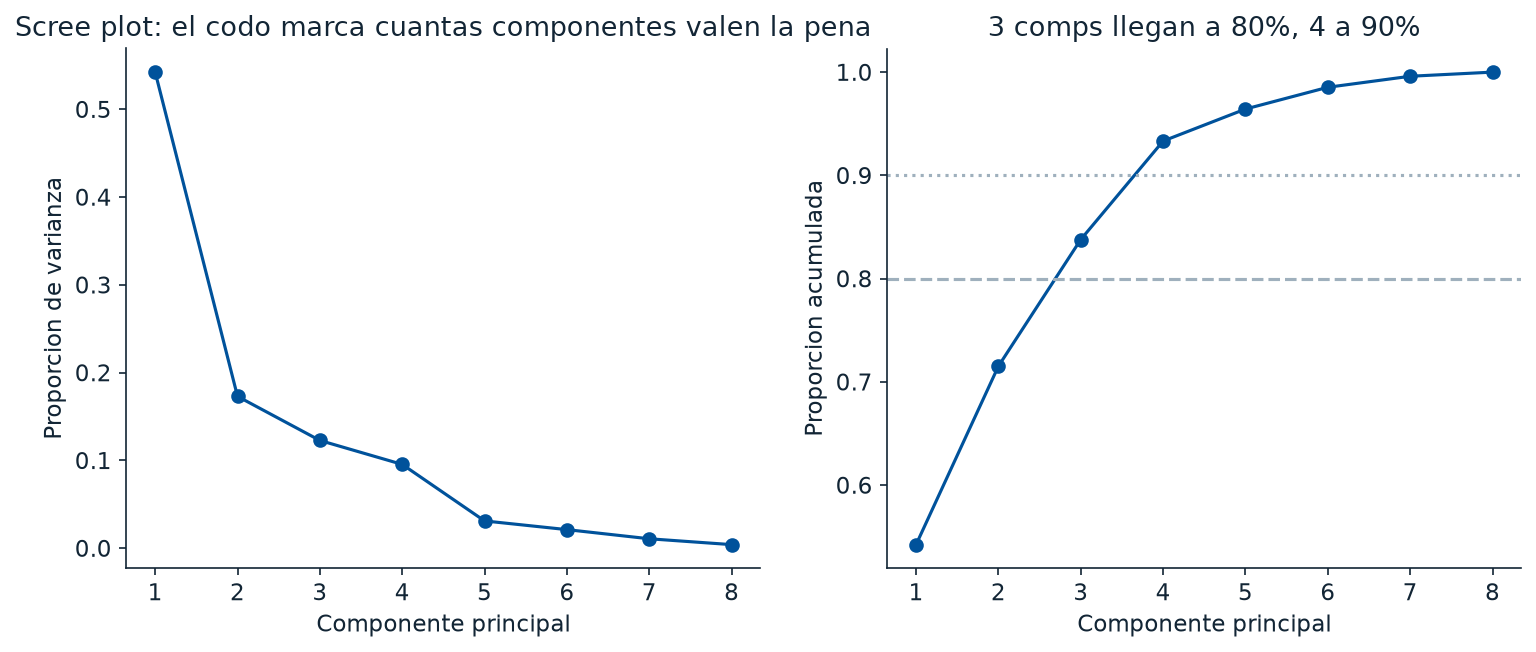
\includegraphics[width=\linewidth,height=0.64\textheight,keepaspectratio]{clase10_scree.png}\\
    {\footnotesize Se busca el \textbf{codo}: el punto donde cada componente adicional deja de aportar. Ac\'a, \alert{3 componentes} llegan al 80\% de la varianza y \alert{4} superan el 90\%.}
\end{frame}

\begin{frame}{La PVE es el $R^2$ de la aproximaci\'on}
    \begin{block}{Un gancho con lo que ya saben}
        La proporci\'on de varianza explicada por las primeras $M$ componentes se interpreta \textbf{exactamente} como el $R^2$ de la regresi\'on lineal: qu\'e fracci\'on de la variabilidad total se logra explicar.
    \end{block}
    \begin{itemize}
        \item Con 2 componentes explicamos el \textbf{71,5\%} de la variabilidad de las ocho variables.
        \item Por eso el biplot en dos dimensiones es una representaci\'on \alert{fiel} del dataset completo.
        \item Y por eso retener componentes es quedarse con la se\~nal y descartar, sobre todo, ruido.
    \end{itemize}
\end{frame}

\begin{frame}{M\'axima varianza y m\'inimo error son lo mismo}
    \begin{itemize}
        \item La varianza total de los datos se reparte en \textbf{dos partes}: lo que capturan las primeras $M$ componentes, m\'as el \textbf{error} de reconstruirlos con esas $M$.
        \item Como la varianza total es un n\'umero \textbf{fijo}, subir una es bajar la otra.
    \end{itemize}
    \vfill
    \begin{alertblock}{La equivalencia, cerrada}
        \textbf{Maximizar} la varianza explicada por las primeras $M$ componentes es \alert{exactamente lo mismo} que \textbf{minimizar} el error de reconstrucci\'on.
    \end{alertblock}
    \vfill
    {\footnotesize Es la raz\'on por la que las dos definiciones del Bloque 2, m\'axima varianza y m\'inima distancia, describen el mismo objeto.}
\end{frame}

\begin{frame}{Cu\'antas retener: no hay respuesta \'unica}
    \begin{itemize}
        \item No existe un criterio objetivo y universal. En an\'alisis no supervisado, la decisi\'on es en parte un \textbf{juicio}.
        \item Se mira el \textbf{codo} del scree plot, o se fija un umbral de varianza acumulada (80\% o 90\%).
        \item Regla pr\'actica: si las primeras componentes no muestran nada interesante, las siguientes tampoco suelen hacerlo.
    \end{itemize}
    \vfill
    \begin{block}{Cuando s\'i hay criterio objetivo}
        Si las componentes se usan como \textbf{predictores} de un modelo posterior, el n\'umero se elige como cualquier hiperpar\'ametro: por \textbf{validaci\'on cruzada}.
    \end{block}
\end{frame}

\begin{frame}{}
    \vfill
    \begin{center}
        \href{https://colab.research.google.com/github/tomdamelio/analitica_de_datos/blob/main/clases/clase-10/notebooks/clase10_python.ipynb}{
\includegraphics[height=7ex]{colab_logo.png}}\\[0.6em]
        {\Large\textbf{A la notebook}}\\[0.6em]
        {\normalsize Reconstruir un dato con 1, 2 y todas las componentes, y ver caer el error.}\\[0.4em]
        {\footnotesize \textbf{Ejercicio:} cu\'antas componentes hacen falta para llegar al 90\%.}
    \end{center}
    \vfill
\end{frame}

%======================= BLOQUE 5 =======================
\section{Decisiones y alcance}
\bloque{tabRed}

\begin{frame}{}
    \vfill
    \begin{center}
        {\small\textbf{\color{tabRed}BLOQUE 5 DE 6}}\\[0.5em]
        {\Large\textbf{Decisiones pr\'acticas y alcance}}\\[0.8em]
        {\normalsize Estandarizar, m\'etodos no lineales y casos aplicados.}
    \end{center}
    \vfill
\end{frame}

\begin{frame}{?`Qu\'e pasa si no estandarizamos?}
    \begin{alertblock}{Antes de mirar el resultado}
        Vamos a correr PCA sobre las ocho variables \textbf{sin estandarizar}. ?`Qu\'e variable creen que va a dominar la primera componente, y por qu\'e?
    \end{alertblock}
    \begin{itemize}
        \item La \textbf{nota de admisi\'on} va de 0 a 200; las materias aprobadas, de 0 a 10.
        \item Sus varianzas: \textbf{210} frente a \textbf{9,6}.
        \item Como PCA busca \alert{m\'axima varianza}, sin estandarizar la escala de medici\'on decide el resultado.
    \end{itemize}
\end{frame}

\begin{frame}{Sin escalar, una variable secuestra PC1}
    \centering
    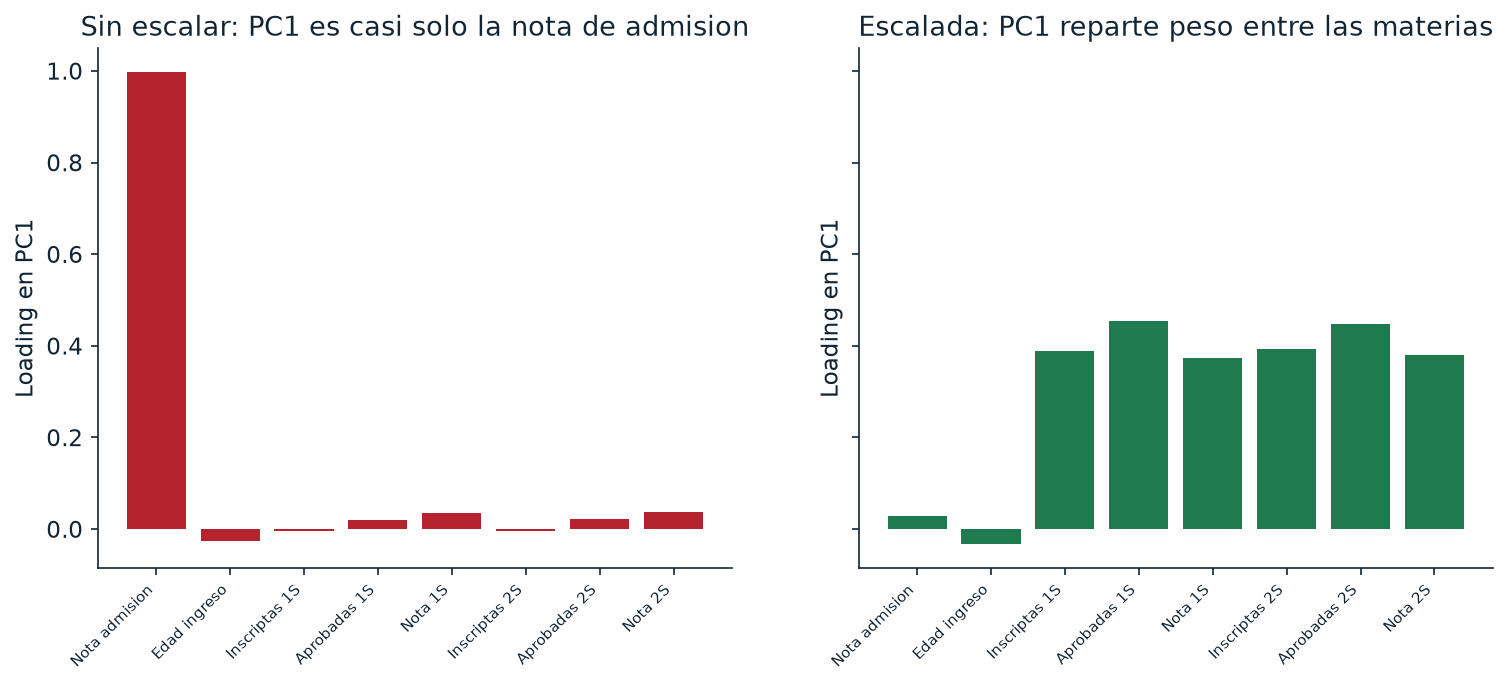
\includegraphics[width=\linewidth,height=0.64\textheight,keepaspectratio]{clase10_escalado.png}\\
    {\footnotesize Pesos de PC1 sin escalar (izquierda) y escalando (derecha). Sin estandarizar, PC1 es \textbf{casi solo la nota de admisi\'on}; estandarizando, reparte peso entre las materias y se vuelve interpretable. \alert{Salvo unidad com\'un, se estandariza siempre.}}
\end{frame}

\begin{frame}{M\'as all\'a de PCA: t-SNE y UMAP}
    \centering
    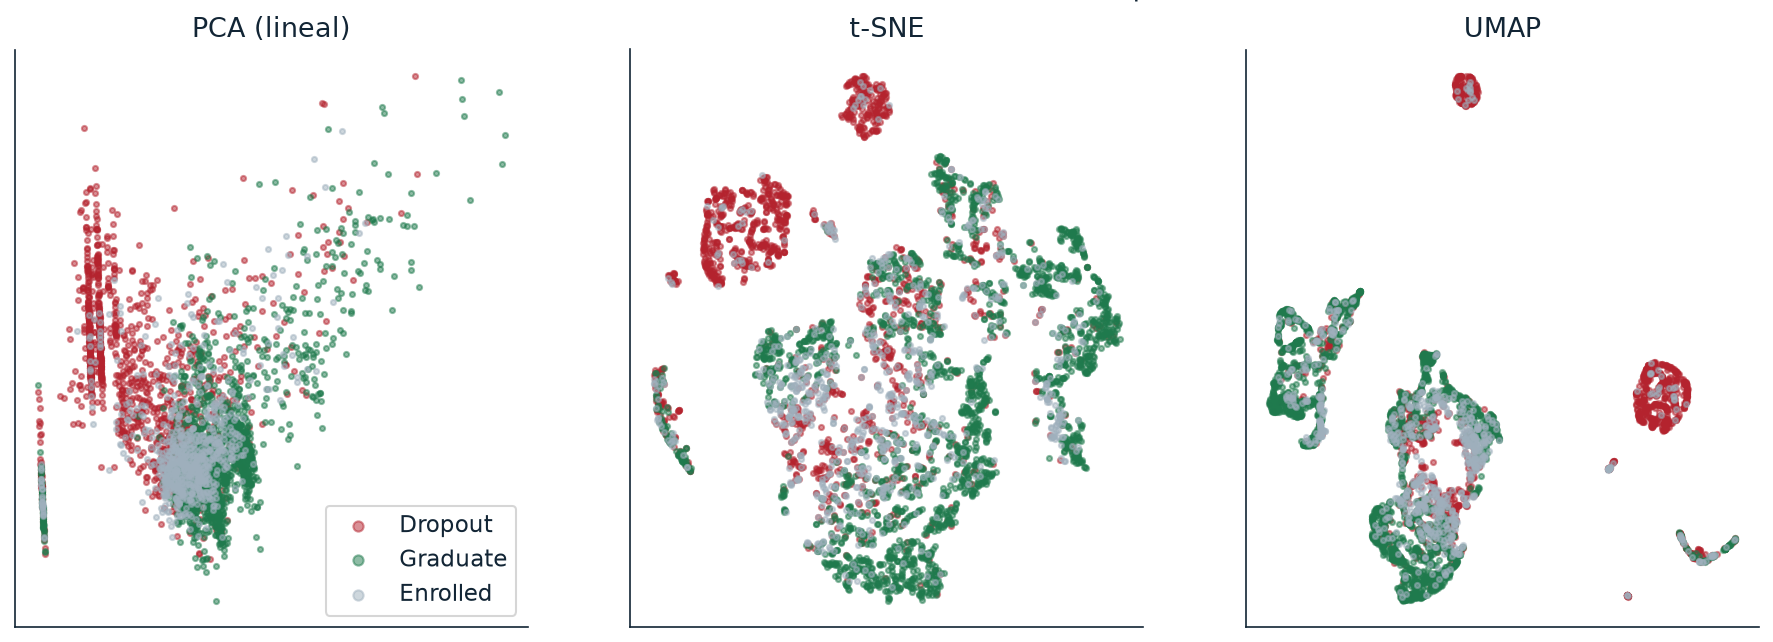
\includegraphics[width=\linewidth,height=0.62\textheight,keepaspectratio]{clase10_no_lineales_notitle.png}\\
    {\footnotesize PCA es \textbf{lineal}: solo captura estructura describible con direcciones rectas. t-SNE y UMAP construyen una vista 2D que preserva sobre todo la \textbf{vecindad local}, y por eso los grupos aparecen mucho m\'as separados.}
\end{frame}

\begin{frame}{Lo que t-SNE y UMAP no garantizan}
    \begin{alertblock}{Tres cuidados}
        \begin{itemize}
            \item \textbf{No preservan distancias globales}: la separaci\'on entre dos grupos lejanos en el dibujo \alert{no es interpretable}.
            \item \textbf{Dependen de hiperpar\'ametros}: cambiar la \emph{perplexity} o el n\'umero de vecinos cambia el gr\'afico.
            \item \textbf{Sus ejes no significan nada}: no hay loadings que interpretar.
        \end{itemize}
    \end{alertblock}
    \begin{itemize}
        \item No est\'an en el cap\'itulo 12 del libro: son un complemento moderno.
        \item Regla: usalos para \textbf{descubrir} grupos, nunca para \textbf{medir} distancias.
    \end{itemize}
\end{frame}

\begin{frame}{PC1 como \'indice: el Nivel Socioecon\'omico}
    \begin{block}{Filmer y Pritchett (2001), \emph{Demography}}
        Para estimar la riqueza del hogar sin datos de gasto, construyeron un \textbf{\'indice} a partir de indicadores de \textbf{posesi\'on de bienes} del hogar, usando PCA para derivar los \alert{ponderadores}.
    \end{block}
    \begin{itemize}
        \item Los hogares se ordenan por su valor en \textbf{PC1} y se agrupan en \textbf{quintiles}, de m\'as pobre a m\'as rico.
        \item Vyas y Kumaranayake (2006) es la gu\'ia metodol\'ogica de referencia sobre c\'omo construirlo e interpretarlo.
        \item \textbf{Punto de discusi\'on:} casi todos estos trabajos usan \emph{solo} PC1. Hay literatura que propone combinar varias componentes, porque PC1 suele explicar una parte modesta de la varianza.
    \end{itemize}
\end{frame}

\begin{frame}{32 medidas de comportamiento, seis dimensiones}
    \begin{block}{Arguello y Crescenzi (2019)}
        Analizaron con PCA hasta \textbf{32 medidas de comportamiento} por sesi\'on (cantidad de b\'usquedas, clics, tiempos de permanencia, scrolls, movimientos del mouse) en estudios de b\'usqueda de informaci\'on.
    \end{block}
    \begin{itemize}
        \item Objetivo: entender qu\'e \textbf{fen\'omenos latentes} capturan esas medidas, y c\'omo influyen en las percepciones posteriores (carga de trabajo, dificultad, \emph{engagement}).
        \item Usaron la matriz de \textbf{correlaci\'on} y no la de covarianza, porque las medidas est\'an en escalas muy distintas: es \alert{el mismo argumento del escalado} que vimos reci\'en.
        \item Para elegir cu\'antas componentes: autovalor \textbf{mayor a 1}, y que cada componente tenga al menos \textbf{dos variables} con pesos altos.
    \end{itemize}
\end{frame}

\begin{frame}{Del componente al modelo}
    \begin{itemize}
        \item Aplicaron una \textbf{rotaci\'on varimax}: redistribuye los pesos para que cada variable cargue fuerte en una sola componente. Facilita \alert{nombrarlas}, y es pr\'actica est\'andar aplicada aunque el libro no la desarrolle.
        \item As\'i nombraron cada dimensi\'on seg\'un qu\'e medidas pesaban en ella, por ejemplo \emph{abandono de b\'usquedas} o \emph{ritmo de interacci\'on}.
        \item Despu\'es usaron los \textbf{scores} de las componentes, en lugar de las 32 medidas originales, como predictores de un modelo de regresi\'on.
    \end{itemize}
    \vfill
    \begin{exampleblock}{El resultado}
        Seis componentes explicaron el \textbf{76\%} de la varianza de las medidas de comportamiento. El circuito completo: comportamiento crudo $\rightarrow$ dimensiones interpretables $\rightarrow$ efectos sobre lo que la gente percibe.
    \end{exampleblock}
\end{frame}

%======================= BLOQUE 6 =======================
\section{Supuestos y l\'imites}
\bloque{tabBrown}

\begin{frame}{}
    \vfill
    \begin{center}
        {\small\textbf{\color{tabBrown}BLOQUE 6 DE 6}}\\[0.5em]
        {\Large\textbf{Supuestos y l\'imites}}\\[0.8em]
        {\normalsize Qu\'e asume PCA, y cu\'ando conviene desconfiar.}
    \end{center}
    \vfill
\end{frame}

\begin{frame}{Qu\'e asume PCA}
    \begin{itemize}
        \item PCA se apoya en la matriz de \textbf{covarianzas o correlaciones} (de Pearson).
        \item Eso trae tres supuestos impl\'icitos sobre las variables:
        \begin{itemize}
            \item que son \textbf{continuas},
            \item que las relaciones entre ellas son \textbf{lineales},
            \item que las distancias entre valores consecutivos son \alert{equiespaciadas}.
        \end{itemize}
        \item El tercero es el que m\'as tensiona en Ciencias del Comportamiento: en una escala de acuerdo, ?`la distancia entre ``en desacuerdo'' y ``neutral'' es la misma que entre ``neutral'' y ``de acuerdo''?
    \end{itemize}
\end{frame}

\begin{frame}{Escalas Likert: cuasi-continuas en la pr\'actica}
    \begin{block}{La pr\'actica est\'andar en psicometr\'ia}
        Con escalas de \textbf{5 o m\'as puntos} (idealmente 7) y una distribuci\'on no muy asim\'etrica, se aplica PCA directamente, tratando la variable ordinal como si fuera continua.
    \end{block}
    \begin{itemize}
        \item El sesgo que introduce suele ser \textbf{chico y manejable}.
        \item As\'i se analiza la enorme mayor\'ia de los cuestionarios de personalidad, actitudes y clima laboral.
        \item Es exactamente lo que hicieron los estudios de Big Five que vimos al principio.
    \end{itemize}
    \vskip0.3em
    {\footnotesize Conviene igual \textbf{declarar} la decisi\'on al reportar: es un supuesto que se asume, no un detalle t\'ecnico invisible.}
\end{frame}

\begin{frame}{Qu\'e conviene evitar}
    \begin{alertblock}{El l\'imite claro}
        Aplicar PCA con correlaciones de Pearson a variables \textbf{nominales}, es decir, sin ning\'un orden: tipo de contrato, carrera, provincia.
    \end{alertblock}
    \begin{itemize}
        \item Si no hay orden, \alert{no hay nada que preservar}: los n\'umeros que codifican las categor\'ias son etiquetas arbitrarias, y las correlaciones que se calculan sobre ellas no significan nada.
        \item El chequeo previo m\'as \'util sigue siendo el m\'as simple: \textbf{mirar la matriz de correlaciones}. Si es casi diagonal, no hay redundancia que explotar y PCA no va a ayudar.
    \end{itemize}
\end{frame}

%======================= CIERRE =======================
\section{Cierre}
\navytheme

\begin{frame}{}
    \vfill
    \begin{center}
        \href{https://colab.research.google.com/github/tomdamelio/analitica_de_datos/blob/main/clases/clase-10/notebooks/clase10_python.ipynb}{
\includegraphics[height=7ex]{colab_logo.png}}\\[0.6em]
        {\Large\textbf{La pr\'actica}}\\[0.6em]
        {\normalsize Aplicar PCA \textbf{+ clustering} sobre el dataset de rotaci\'on de personal que ya conocen,}\\
        {\normalsize para descubrir \alert{perfiles latentes} de empleados.}
    \end{center}
    \vfill
\end{frame}

\begin{frame}{Los perfiles son hip\'otesis, no verdades}
    \centering
    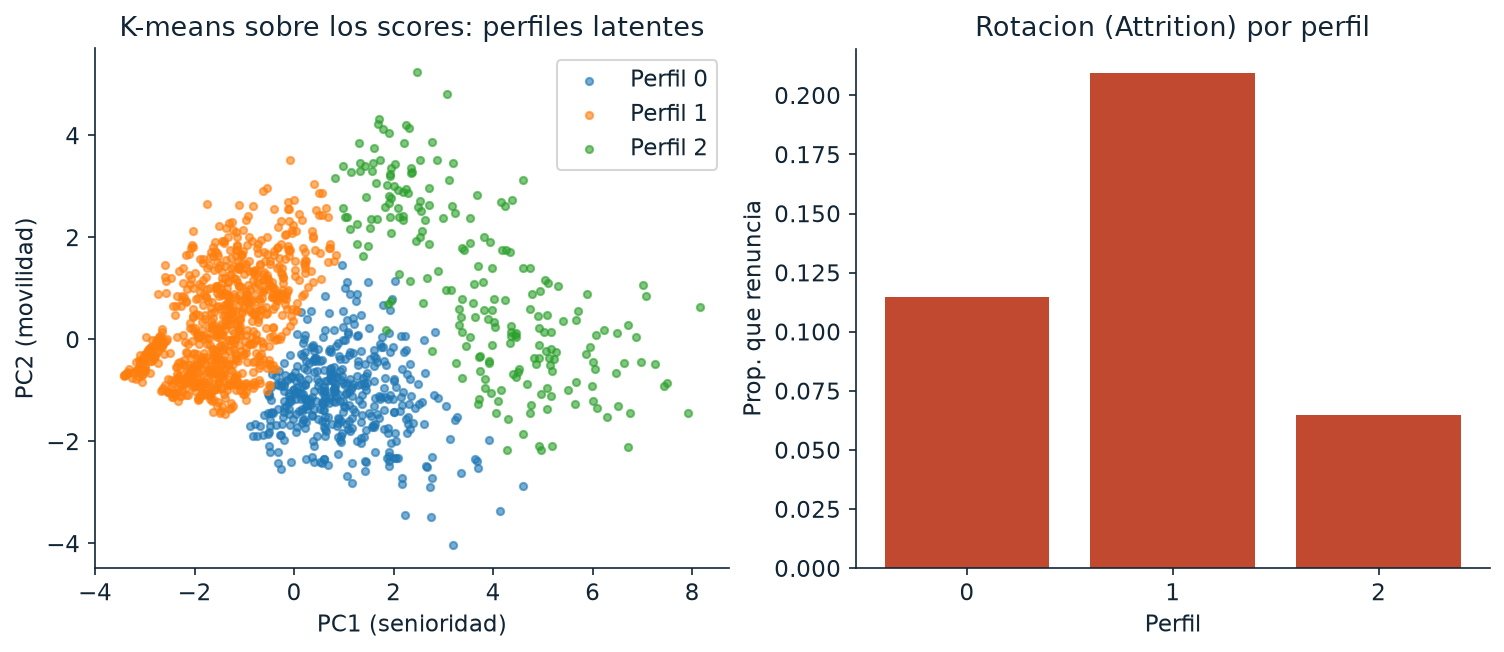
\includegraphics[width=\linewidth,height=0.58\textheight,keepaspectratio]{clase10_perfiles.png}\\
    {\footnotesize Clusters sobre los primeros scores, y su tasa de rotaci\'on. El clustering \textbf{no es robusto}: cambia con la estandarizaci\'on, con cu\'antas componentes se retienen y con $k$. Conviene repetirlo con distintas opciones y quedarse con lo que \alert{persiste}.}
\end{frame}

\begin{frame}{Ya pod\'es...}
    \begin{itemize}
        \item Explicar por qu\'e muchas variables correlacionadas se resumen en pocas dimensiones.
        \item Interpretar \textbf{loadings} y \textbf{scores}, y leer un \textbf{biplot} con sus tres criterios.
        \item Decidir cu\'ando \textbf{estandarizar} y cu\'antas componentes \textbf{retener}.
        \item Reconocer qu\'e aportan y qu\'e no los m\'etodos no lineales, y qu\'e asume PCA.
    \end{itemize}
    \vfill
    \begin{block}{El hallazgo de hoy, en una frase}
        Sin haber visto nunca la etiqueta de deserci\'on, la \textbf{primera componente} de ocho variables acad\'emicas result\'o ser un \alert{eje de riesgo} que separa a quienes abandonan de quienes se grad\'uan.
    \end{block}
    \vfill
    {\footnotesize \textbf{Lo que viene:} representar textos en pocas dimensiones, con \emph{embeddings} (Clases 11 y 12).}
\end{frame}

\end{document}
